\documentclass[a4paper,11pt]{report}
\usepackage[utf8]{inputenc}
\usepackage[francais]{babel}
\usepackage{graphicx}
\usepackage{epsf}
\usepackage{epsfig}
\usepackage{listings}
\usepackage{color}
\usepackage{graphicx}
\usepackage{wrapfig}
\usepackage{caption}
\usepackage{subcaption}
\definecolor{dkgreen}{rgb}{0,0.6,0}
\definecolor{gray}{rgb}{0.5,0.5,0.5}
\definecolor{mauve}{rgb}{0.58,0,0.82}
\usepackage{amssymb}
\setcounter{tocdepth}{5}
\setcounter{secnumdepth}{5}
\providecommand{\keywords}[1]{\textbf{\textit{Index terms---}} #1}
\usepackage{geometry}
\geometry{ hmargin=2.5cm, vmargin=2.5cm } 
\setcounter{tocdepth}{5}
\lstset{frame=tblr,
  language=Python,
  aboveskip=3mm,
  belowskip=3mm,
  showstringspaces=false,
  columns=flexible,
  basicstyle={\small\ttfamily},
  numbers=left,
  numberstyle=\tiny\color{gray},
  keywordstyle=\color{blue},
  commentstyle=\color{dkgreen},
  stringstyle=\color{mauve},
  breaklines=true,
  breakatwhitespace=true,
  tabsize=3
}
\newcommand{\bigO}[1]{\ensuremath{\mathop{}\mathopen{}O\mathopen{}\left(#1\right)}}
\pagestyle{plain}



\begin{document}

~\\\\\\\\\\
\begin{center}
\mbox{\huge RAPPORT de l'UE : RI - Recherche d'informations}\\~\\ \mbox{ }\\ \textbf{\LARGE Création d'un moteur de recherche}
\end{center}~\\
\begin{center}\large Paul Willot et Florian Toqué\end{center}
\begin{center}\large 9 Novembre 2015 \end{center}~\\\\\\\\\\\\\\\\\
%\rule{\linewidth}{.1pt}
%\begin{center}Abstract\end{center}
\begin{center}\textbf{\Large{Résumé}}\end{center}
\large{Ce rapport aborde les différentes étapes que nous avons suivies pour créer un moteur de recherche. Différents algorithmes de recherche d'informations seront notamment expliqués dans ce rapport.}\\\\\\\\\\\\\\\\\\\\\\\\
\rule{\linewidth}{.5pt}
\textsc{Mots-clés:}\\
Moteur de recherche --- Page Rank --- Hits --- Modèle vectoriel --- Indexation\\\\\\



\newpage
\tableofcontents







\chapter*{{\centering Introduction}}
\addcontentsline{toc}{chapter}{Introduction}
Les moteurs de recherche servent à retrouver de l'information parmi un ensemble de documents. Pour chaque requête posée, leur action est de retourner les documents les plus pertinents. Le temps de réponse est aussi important pour juger si un moteur de recherche est performant ou non. Nous avons créer au cours des 6 TME (travaux machine encadrés de 2 heures) de l'UE RI un moteur de recherche. Les différentes parties de ce rapport vont porter sur chacun des TMEs. Nous allons donc expliquer ce qu'est l'indexation de documents, le modèle vectoriel qui est un algorithme de recherche d'information. Par la suite nous évoquerons comment nos modèles sont évalués ainsi que d'autres modèles qui sont probabilistes. Puis nous parlerons de l'algorithme du Page Rank qui a fait la notoriété de Google et plus généralement des algorithmes de marche aléatoire.  Enfin nous expliquerons différentes méthodes de combinaisons de scores qui permettent de tirer profit de différents modèles.
A noter que pour chaque modèle nous nous intéresserons à l'optimisation des paramètres, qui permet aux algorithmes d'obtenir de meilleures performances quant à leurs évaluations.



\section*{1.Indexation}
\addcontentsline{toc}{section}{1.Indexation}
Par soucis de temps et de mémoire, il est nécessaire d'indexer les documents du corpus. Les indexes permettent de ne pas devoir relire pour chaque requête, l'intégralité du corpus. Par ailleurs ils permettent d'obtenir l'information sur un document en \bigO{1}.
\subsection*{1.Collections de documents}
\addcontentsline{toc}{subsection}{1.Collections de documents}
Nous avons travaillé sur deux corpus comportant plusieurs requêtes ainsi que les documents pertinents trouvées par des humains. Ces réponses se structurent sous forme de liste comprenant le numéro des documents en lien avec la requête. Le corpus CACM regroupe des résumés d'articles provenant de la partie communication du journal ACM. Ce corpus compte 4204 textes et 64 requêtes. Le corpus CISI comporte 2460 textes et 112 requêtes.
\subsection*{2.Transformation des textes}
\addcontentsline{toc}{subsection}{2.Transformation des textes}
Avant d'analyser les textes nous avons appliqué pour chacun d'entre eux un algorithme de stemmatisation permettant d'avoir une structure unifiée entre chaque texte. Cette transformation consiste à garder la racine de chaque mot et de supprimer les suffixes. Les mots de chaque requête sont ainsi trouvés parmi les documents, peu importe leurs suffixes.
\subsection*{3.L'indexation}
\addcontentsline{toc}{subsection}{3.L'indexation}

L'indexation s'est faite en deux étapes. Premièrement nous avons créé un index par document c'est à dire que pour chaque documents nous avons calculé le nombre de fois ou chaque mot apparaît. Le deuxième index que nous avons créé sert à calculer pour chaque mot de l'ensemble du corpus l'ensemble des documents dans lequel il apparaît ainsi que son nombre d'apparition dans ceux-ci. Ces indexes sont enregistrés dans des fichiers \textbf{random access file} pour une plus grande rapidité d'accès à l'information.

\section*{2.Modèle vectoriel}
\addcontentsline{toc}{section}{2.Modèle vectoriel}

Le modèle vectoriel est un algorithme de recherche d'informations permettant de transformer un document ou une requête sous forme de vecteurs et pouvoir ainsi calculer la similarité entre un document et une requête en utilisant la similarité cosinus entre ces deux représentations. L'autre méthode pour calculer la similarité entre un document et une requête est de les représenter avec une pondération pour chaque mot et de faire le produit vectoriel entre les deux. Différents calculs de pondérations ont été appliqués, la plus connue étant celle du TF-IDF qui est le calcul de la fréquence de chaque mot divisé par la fréquence d'apparition du mot dans le corpus entier, pour donner moins d'importance aux mots présents très souvent tels que les déterminants. 



\section*{3.Evaluation des résultats}
\addcontentsline{toc}{section}{3.Evaluation des résultats}
Pour chaque requête une liste de documents pertinents a été trouvé manuellement, ainsi une évaluation des résultats est possible. Pour connaître la performance de notre moteur de recherche différentes mesures sont applicables. Nous avons utilisé la mesure Précision-Rappel et la précision moyenne.

\subsection*{1.La mesure Précision-Rappel}
\addcontentsline{toc}{subsection}{1.La mesure Précision-Rappel}
Le rappel est ainsi calculé:\\\\
$Rappel_k = \frac{documents~pertinents~attribu\acute{e}s~au~rang~k}{nombre~de~documents~pertinents}$\\\\\\

La précision est ainsi calculée:\\\\
$Pr\acute{e}cision_k = \frac{documents~pertinents~attribu\acute{e}s~au~rang~k}{k}$ 

\subsection*{2.La mesure de précision Moyenne}
\addcontentsline{toc}{subsection}{2.La mesure de précision Moyenne}

La précision moyenne se calcule sur l'ensemble des précisions obtenues après chaque document pertinent. 






\section*{4.Modèles probabilistes}
\addcontentsline{toc}{section}{4.Modèles probabilistes}

Au contraire du modèle vectoriel, il n'est pas nécessaire de transformer l'espace des documents sous forme de vecteurs. La similarité entre un document et une requête est calculée à l'aide de formules probabilistes.

\subsection*{1.Modèle de langue}
\addcontentsline{toc}{subsection}{1.Modèle de langue}
La similarité entre une requête \textbf{q} et un document \textbf{d} pour le modèle de langue se calcule ainsi:\\\\
 $f(d,q)=\sum_{t \in q } tf(t,q) log( \lambda p_{M_d} (t)+(1- \lambda )p_{M_c} (t)))$\\\\ Où  $p_{M_d}(t)$ correspond à la probabilité de rencontrer le mot \textbf{t}  dans le document \textbf{d} et  $p_{M_c}(t)$ la probabilité de rencontrer le mot \textbf{t} parmi l'ensemble des documents du corpus.
 
\subsection*{2.Modèle BM25 - OKAPI}
\addcontentsline{toc}{subsection}{2.Modèle BM25 - OKAPI}

Le modèle de langue OKAPI est une fonction qui permet de d'ordonner selon leurs pertinences un ensemble de documents, cette fonction se base sur l'apparition des termes de la requête dans chaque documents, en considérant que les mots de chaque document sont indépendants entre eux.

Le score de similarité entre une requête \textbf{q} et un document \textbf{d} pour le modèle OKAPI est:\\\\
$f(d,q)=\sum_{t\in q}idf'(t)\frac{(k_1+1)tf(t,d)}{k_1((1-b)+bL(d)/L_{moy})+tf(t,d)}$\\\\
Où k1 est entre 1 et 2, et $b\approx0.75$



\section*{5.Marche aléatoires sur les graphes}
\addcontentsline{toc}{section}{5.Marche aléatoires sur les graphes}
Sur le web, les pages sont considérées comme des documents, ces pages sont reliés entre elles par des liens. Pour chaque page il existent donc des liens sortants et des liens entrants. Ces liens entre documents forment donc un graphe. Les corpus CACM et CISI que nous utilisons contiennent des fichiers de relations permettant d'appliquer des algorithmes de marche aléatoires. Le principe de ces algorithmes repose sur le fait que plus un document a de document qui pointe vers celui-ci, plus ce document est important. Ces algorithmes permettent donc de choisir les documents les plus important parmi un ensemble de documents liés à une requête, cet ensemble de documents est initialement trouvé grâce a un algorithme de recherche d'information cité avant (modèle vectoriel ou probabiliste).

\subsection*{1.Page Rank}
\addcontentsline{toc}{subsection}{1.Page Rank}
Le page rank est l'algorithme qui a fait la notoriété du moteur de recherche Google. Le principe est de partir d'un ensemble \textbf{V} de documents censés être pertinents pour une requête, puis de faire naviguer un "surfeur" à partir d'un des documents de \textbf{V} à travers le graphe. Une fois que l'algorithme se termine(nombre n d'itérations ou convergence de l'algorithme), les documents avec la plus grande probabilité d'apparition correspondent aux documents avec le meilleur score de similarité.

\subsection*{2.HITS}
\addcontentsline{toc}{subsection}{2.HITS}
L'algorithme de HITS repose sur l'identification de deux types de documents, les autorités(pages ayant beaucoup de liens entrants) et les hubs(pages ayant beaucoup de liens sortants). Les scores de chacun se renforcent mutuellement, après convergence les documents les plus pertinents sont ceux ayant leurs scores d'autorité le plus haut.











\section*{6.Combinaison des scores}
\addcontentsline{toc}{section}{6.Combinaison des scores}

Le principe est de créer un classifieur linéaire qui nous permet de savoir si un document est pertinent ou non. Pour chaque document les features prisent en compte sont le score de chacun des modèles. D'autres features peuvent être prisent en compte tel que la longueur, la somme des idfs de la requête et des documents. La labellisation des documents se faisant pour chaque requête à l'aide de la liste des documents pertinents trouvés manuellement.

\section*{7.Optimisation des paramètres}
\addcontentsline{toc}{section}{7.Optimisation des paramètres}
Les optimisation ont été fait en cross validation (ensemble de test et un ensemble de train) pour le corpus CACM.\\
Nous avons optimisé le paramètre lambda du modèle de langue à l'aide d'un grid search.\\
 \begin{center}
 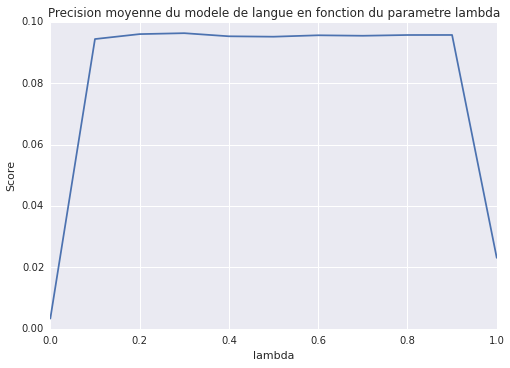
\includegraphics[width=0.7\textwidth]{lambdaLM}
\end{center}

Nous avons optimisé le paramètre k du modèle OKAPI à l'aide d'un grid search.\\
 \begin{center}
 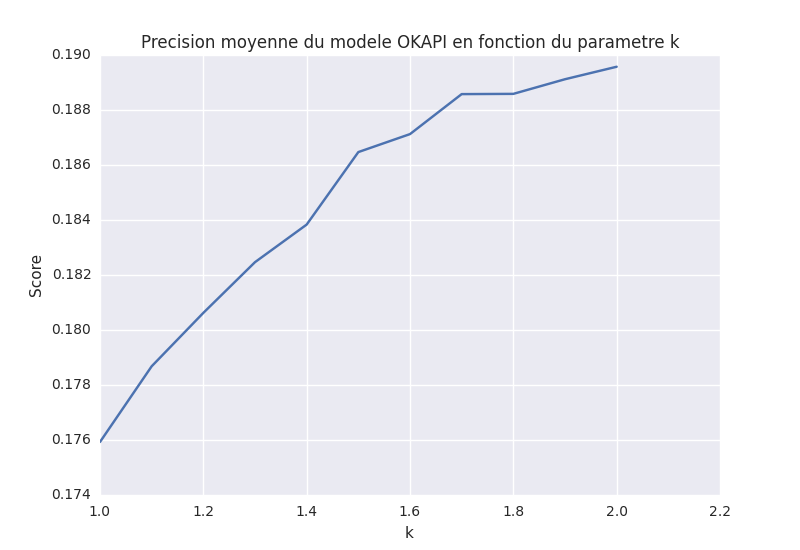
\includegraphics[width=0.7\textwidth]{k_OKAPI}
\end{center}








%\section*{7.Comparaison des scores entre différentes mesures}
%\addcontentsline{toc}{section}{7.Comparaison des scores entre différentes mesures}











\chapter*{Conclusion}
\addcontentsline{toc}{chapter}{Conclusion}
Nous avons programmé l'ensemble du moteur de recherche en Scala, hormis la partie Parser et Stemmatisation faites en Java. Ce projet nous a donc permit d'apprendre à maîtriser un langage en plus des connaissances statistiques et algorithmiques utilisées dans la mise en place d'un moteur de recherche. 





%\section*{1.Nom\_section}
%\addcontentsline{toc}{section}{1.Nom\_section}

%\subsection*{1.Nom\_subsection}
%\addcontentsline{toc}{subsection}{1.Nom\_subsection}

%\subsubsection*{1.Nom\_subsubsection}
%\addcontentsline{toc}{subsubsection}{1.Nom\_subsubsection}





%ajouter des images png \hfill si ajout d'une autre photo à côté
%\includegraphics[width=0.5\textwidth]{nom_image}\hfill
%\includegraphics[width=0.5\textwidth]{nom_image}



\end{document}
